\subparagraph{Задание 4.6 (2)}

\textbf{Условие}:
Выполнить программу по шагам, нажимая клавишу \textbf{F7}, до конца. Проcмотреть содержимое экрана (\textbf{Alt} + \textbf{F5}). После какой операции ассемблера на экране появляются строки?
 
\textbf{Решение}:

Выполняю программу нажимая клавишу \textbf{F7}.

Просматриваю консоль клавишами \textbf{Alt} + \textbf{F5}.

Далее выполняю программу нажимая клавишу \textbf{F7}.

Просматриваю консоль клавишами \textbf{Alt} + \textbf{F5}.

Далее выполняю программу нажимая клавишу \textbf{F7}.

Просматриваю консоль клавишами \textbf{Alt} + \textbf{F5}.

Так до тех пор пока не пройдем команду \textbf{int 21h}: вызовится прерывание DOS и появится вывод в консоль.

Turbo Debugger по нажатию \textbf{F7} на рисунке \ref{fig:task_4_6_2__F7} (стр. \pageref{fig:task_4_6_2__F7}).

Turbo Debugger по нажатию \textbf{Alt} + \textbf{F5} на рисунке \ref{fig:task_4_6_2__Alt_F5} (стр. \pageref{fig:task_4_6_2__Alt_F5}).

\begin{figure}[!htp]
    \centering
    \begin{minipage}{0.48\textwidth}
        \centering
        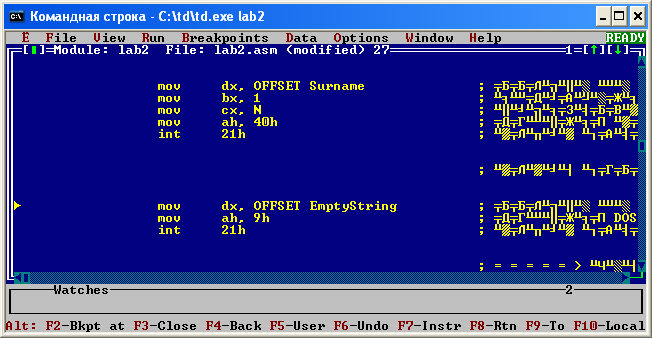
\includegraphics[width=.98\linewidth]
            {../_INCLUDES/task-4-6-2/F7.png}
        \caption{Нажимаю \textbf{F7}\\в Turbo Debugger}
        \label{fig:task_4_6_2__F7}
    \end{minipage}
    \begin {minipage}{0.48\textwidth}
        \centering
        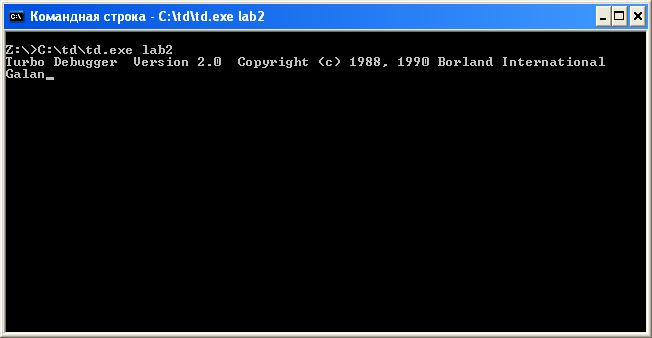
\includegraphics[width=.98\linewidth]
            {../_INCLUDES/task-4-6-2/Alt+F5.png}
        \caption{Нажимаю \textbf{Alt} + \textbf{F5}\\в Turbo Debugger}
        \label{fig:task_4_6_2__Alt_F5}
    \end{minipage}
\end{figure}
